% \section{Experimental Results}
\subsection{End-to-end evaluation}
\label{sec:results_e2e}
%\begin{table*}[!htbp]
\small
\centering
\caption{
End-to-end performance of \methodname on Llama-3-8B as a function of the error budget $\epsilon$.
For each $\epsilon$, layer-wise ranks are selected using the precomputed error surfaces, inducing a KV-cache compression ratio (reported in the table).}
\label{tab:main_results}
\resizebox{0.8\textwidth}{!}{%
\begin{tabular}{l c c cc ccc}
\toprule
\multirow{2}{*}{Method} & \multirow{2}{*}{$\epsilon$} & \multirow{2}{*}{KV cache (rel.) $\downarrow$} 
& \multicolumn{2}{c}{Perplexity $\downarrow$} 
& \multicolumn{3}{c}{Zero-shot Acc. $\uparrow$} \\
\cmidrule(lr){4-5}\cmidrule(lr){6-8}
& & & WikiText & C4 & HellaSwag & PIQA & MMLU \\
\midrule
FP16 (no compression) & -- & 1.00 & 7.79 & 18.05 & 0.60 & 0.79 & 0.62 \\
\midrule
 & 0.015 & 0.85 & 9.96 & 24.58 & 0.58 & 0.79 & 0.60  \\
 & 0.030 & 0.76 & 10.22 & 26.78 & 0.57 & 0.78 & 0.56 \\
\methodname & 0.045 & 0.67 & 11.07 & 33.10 & 0.53 & 0.76  & 0.47 \\
 & 0.060 & 0.61 & 12.04 & 40.06 & 0.49 & 0.75 & 0.40 \\
 & 0.090 & 0.57 & 13.06 & 45.67 & 0.46 & 0.74 & 0.37 \\
\bottomrule
\end{tabular}%
}
\end{table*}

We evaluate KV-cache compression on Llama-3-8B using both language modeling (perplexity) and zero-shot multiple-choice benchmarks (accuracy). For \methodname, we sweep the global distortion budget $\epsilon$ used to select layer-wise ranks from the precomputed error surfaces (Sec.~\ref{sec:method}), which induces different KV-cache compression ratios. 
For EigenAttention, we follow the layer-wise threshold selection procedure of \citet{saxena2024eigenattention}: a per-layer SVD threshold $\epsilon_{\mathrm{th}}$ is decreased in fixed steps until the decoder-layer output error meets the target budget, yielding the corresponding ranks and KV cache ratio.

Table~\ref{tab:main_results} reports \methodname results as $\epsilon$ varies. 
As expected, looser budgets induce more aggressive compression (KV-cache ratio decreases from $0.85$ to $0.57$) and degrade both perplexity and downstream accuracy.
Perplexity increases smoothly as the KV cache shrinks, but the degradation is markedly stronger on C4 than on WikiText: for example, moving from KV cache ratio $0.85$ to $0.61$ raises WikiText perplexity from $9.96$ to $12.04$ ($+2.08$), while C4 increases from $24.58$ to $40.06$ ($+15.48$), suggesting that broader-domain modeling is more sensitive to layer-output compression. 
At moderate compression (retaining $0.76$--$0.67$ of the original KV cache), \methodname matches the FP16 baseline on PIQA, while HellaSwag and MMLU degrade more noticeably, indicating task-dependent sensitivity to decoder-layer output perturbations.
At stronger compression (KV$\le 0.61$), drops become substantial across all metrics.

% , indicating that maintaining decoder-layer output preservation becomes increasingly difficult as effective per-head ranks shrink.


We compare \methodname with EigenAttention in Figs.~\ref{fig:accuracy_fig}--\ref{fig:ppl_fig}: we impose the same error budgets $\epsilon$ across the two methods and compare the performance-memory tradeoff of the two approaches.

Across all evaluated KV-cache ratios, \methodname consistently achieves a better performance--memory tradeoff than EigenAttention, improving both zero-shot accuracy and language-model perplexity at a comparable KV-cache footprint.
On zero-shot benchmarks (Fig.~\ref{fig:accuracy_fig}), \methodname outperforms EigenAttention on HellaSwag, PIQA, and MMLU, with the largest gains on MMLU once the KV cache ratio drops below $0.7$; at a matched footprint, \methodname improves MMLU accuracy by $5.4$\%.
On language modeling (Fig.~\ref{fig:ppl_fig}), \methodname yields lower perplexity on both C4 and WikiText-2 across the entire budget range, with the only exception being WikiText-2 at very mild compression (KV-cache ratio $\gtrsim 0.90$). At iso-footprint, \methodname reduces C4 perplexity by $11.9$ points, indicating that directly optimizing decoder-layer output reconstruction error translates into stronger end-to-end quality at iso-memory.


\begin{figure}[ht]
    \centering
    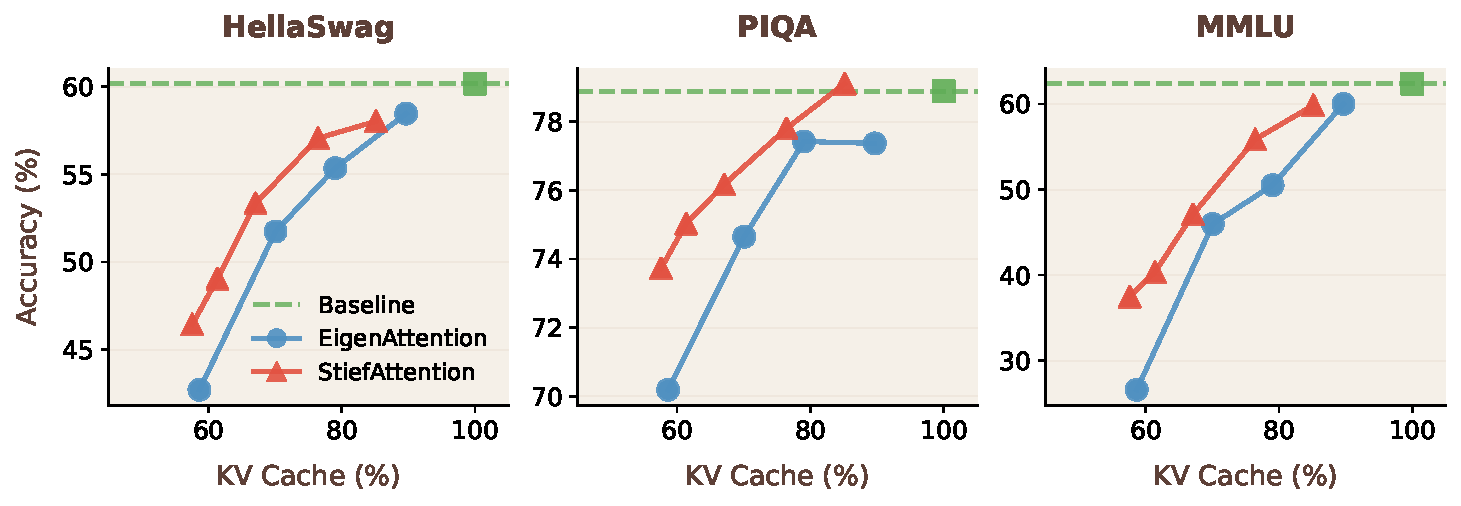
\includegraphics[width=\linewidth]{images/accuracy_tasks_512_2048.pdf}
    \caption{Zero-shot accuracy--memory tradeoff under KV-cache compression on HellaSwag, PIQA, and MMLU. Each point corresponds to an error budget $\epsilon$ that determines layer-wise ranks; the x-axis reports the resulting KV-cache ratio (lower is better).}
    \label{fig:accuracy_fig}
\end{figure}

\begin{figure}[ht]
    \centering
    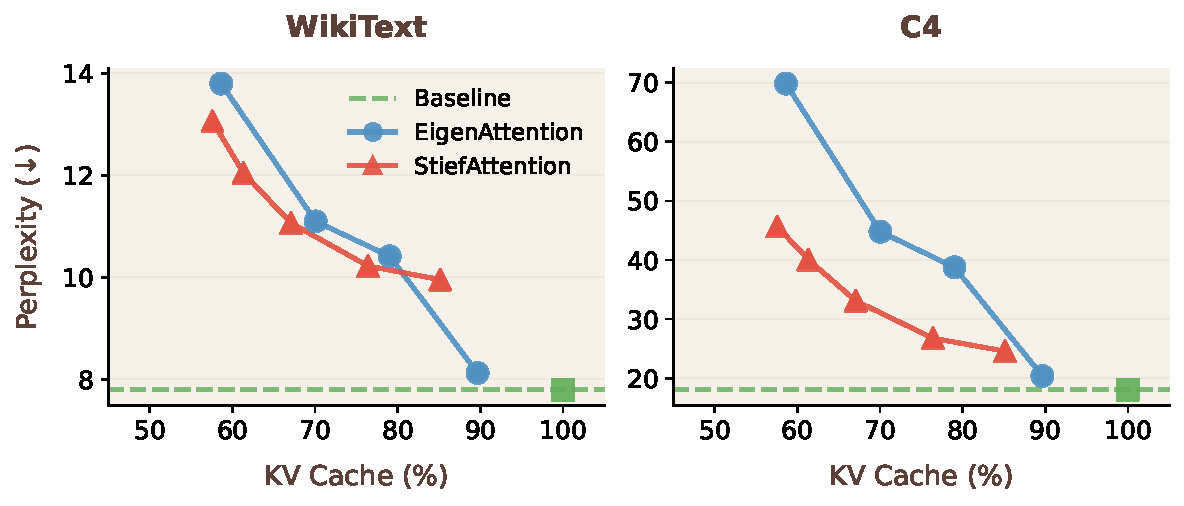
\includegraphics[width=\linewidth]{images/perplexity_tasks_512_2048.pdf}
    \caption{Perplexity--memory tradeoff under KV cache compression on WikiText-2 and C4. Each point corresponds to an error budget $\epsilon$ that determines layer-wise ranks; the x-axis reports the resulting KV cache ratio (lower is better).}
    \label{fig:ppl_fig}
\end{figure}


\subsection{Rank allocation policies}\label{sec:results_policies}
We compare the three rank-allocation policies introduced in Sec.~\ref{sec:method}: \textit{Uniform} (fixed ranks in all layers), \textit{Pareto} (minimum $r_K{+}r_V$ among Pareto-optimal points under $\epsilon$), and \textit{Weighted Pareto} (tighter budgets in early/late layers).
Notice that since \methodname learns projection bases independently of rank selection and precomputes per-layer error surfaces $\Delta_\ell(r_K,r_V)$, rank allocation can be changed at deployment time without retraining the bases.

\paragraph{End-to-end impact.}
Figure~\ref{fig:policies_tradeoff} shows end-to-end performance for each policy as a function of the achieved KV-cache ratio. We report one representative language-modeling metric (WikiText-2 perplexity) and one representative downstream benchmark (PIQA). Depth-adaptive policies consistently improve the performance--memory tradeoff over \textit{Uniform} on both metrics, and \textit{Weighted Pareto} provides a small but consistent gain over \textit{Pareto} across most of the budget range. These results suggest that, given fixed bases, allocating rank non-uniformly across depth is crucial.

\begin{figure}
    \centering
    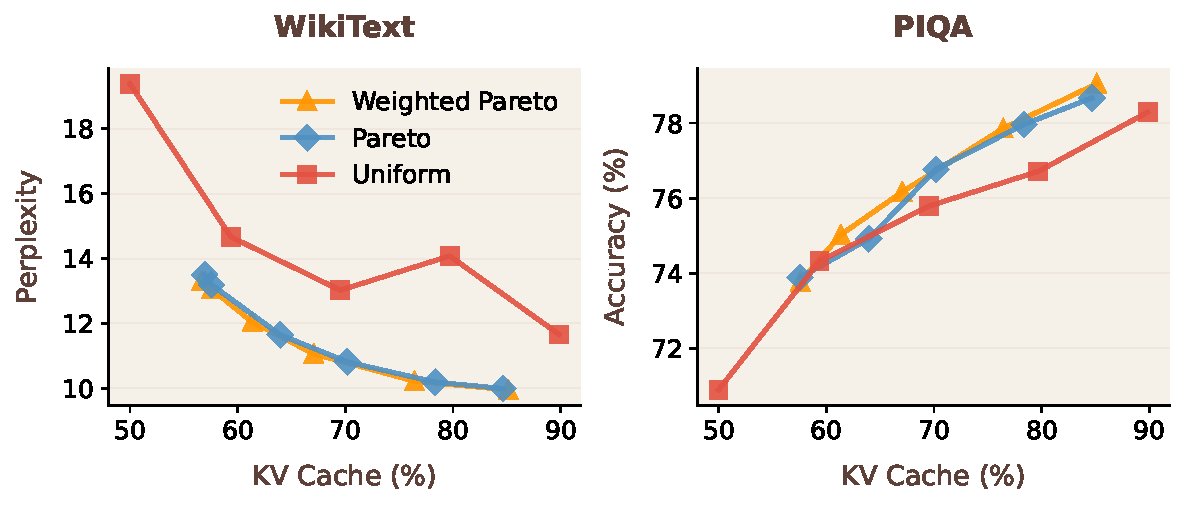
\includegraphics[width=\linewidth]{images/policy_comparison.pdf}
    \caption{Effect of rank-allocation policies.} %We report (left) WikiText-2 perplexity and (right) PIQA zero-shot accuracy as a function of the achieved KV cache ratio.}
    \label{fig:policies_tradeoff}
\end{figure}

\begin{figure}
    \centering
    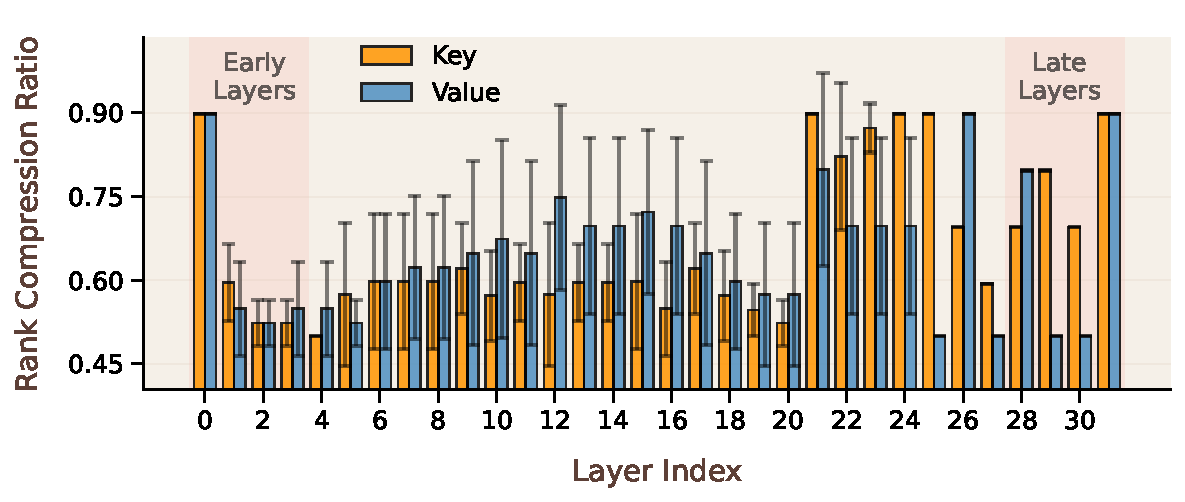
\includegraphics[width=\linewidth]{images/rank_distribution.pdf}
    \caption{Layer-wise rank profiles under Weighted Pareto rank-allocation policy across all error budgets $\epsilon$}
    \label{fig:policies_ranks}
\end{figure}



\paragraph{Where the ranks go.}
Figure~\ref{fig:policies_ranks} summarizes how the best-performing policy (\textit{Weighted Pareto}) distributes rank across depth. Across all evaluated distortion budgets $\epsilon$ in Table~\ref{tab:main_results} (and thus across all induced KV-cache ratios), we record the selected ranks $(r_K, r_V)$ per layer and report their average profile. The y-axis shows the normalized retained rank ($r/d_h$), i.e., the fraction of the original per-head dimension preserved after compression (higher means less compression).
Three trends stand out.
First, the retained rank is highest in early layers and increases again toward deeper layers, with the rise beginning already around the final third of the network rather than only in the last few layers.
Second, values consistently retain a larger fraction of their original dimension than keys.
This reflects that the value pathway is empirically harder to compress under our layer-output distortion criterion: within the same layer, the selected $(r_K,r_V)$ balances key- and value-induced error contributions in $\Delta_\ell(r_K,r_V)$, and the optimizer tends to allocate more capacity to $V$ to maintain decoder-layer output reconstruction quality.
Third, the error bars indicate that different error budget configurations agree on allocating higher ranks to early and late layers, while intermediate layers admit more variation.


\subsection{Why \methodname improves end-to-end performance}
\label{sec:results_analysis}
\begin{figure*}[htp!]
    \centering
    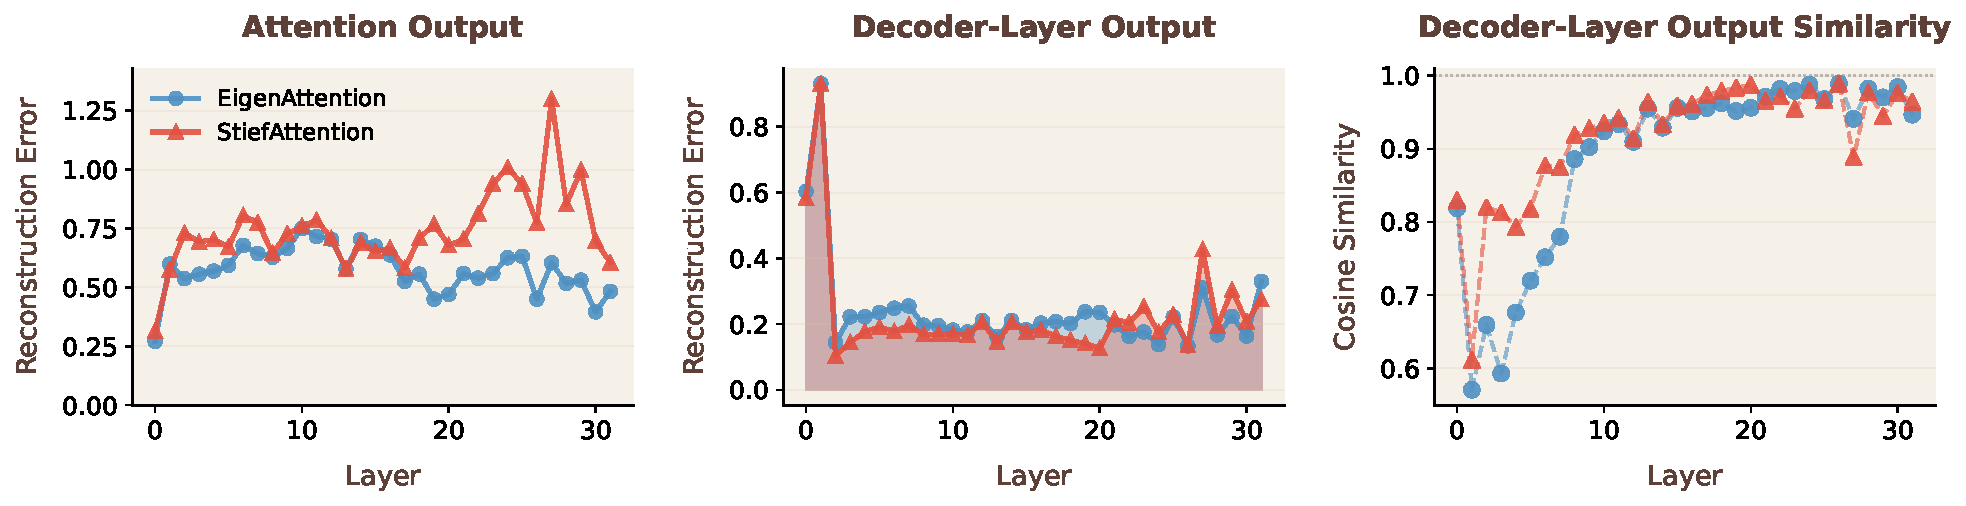
\includegraphics[width=\linewidth]{images/basis_comparison.pdf}
    \caption{Layer-level output preservation diagnostics. We report (i) attention output reconstruction error, (ii) decoder-layer output reconstruction error $\Delta_\ell$, and (iii) cosine similarity between original and compressed decoder-layer outputs.}
    \label{fig:bases_comparison}
\end{figure*}

We analyze \emph{where} \methodname improves reconstruction by measuring layer-wise output preservation on 64 WikiText-2 sequences (2048 tokens). We report results at $(r_K, r_V)=(512,512)$ (half of the original per-head dimension) and observe similar trends across other ranks. For each layer, we log $Q,K,V$, the attention output, and the full decoder-layer output, and compare reconstructions using relative Frobenius-norm error (magnitude) and mean token-wise cosine similarity (direction); Fig.~\ref{fig:bases_comparison} summarizes the results.

As expected, EigenAttention is more robust on proxy targets: it reconstructs intermediate attention quantities more accurately, reducing attention-output error by \textbf{29.6\%} relative to \methodname, with the largest advantage in deeper layers. However, this improvement does not translate to end-to-end behavior. On the decoder-layer output, \methodname achieves lower reconstruction error (\textbf{5.2\%} relative improvement) and, crucially, higher directional agreement (\textbf{+3.3\%} cosine similarity). The cosine gap is most pronounced in early layers: EigenAttention often matches output magnitude but yields activations that are less aligned with the original direction, suggesting that a Frobenius-optimal reconstruction subspace can be misaligned with what downstream nonlinear blocks amplify (softmax/value mixing, residual pathways, normalization, and the MLP).

Overall, these results support the paper’s main claim: proxy reconstruction objectives can accurately preserve intermediate attention quantities while still missing the output-relevant subspace, whereas \methodname directly optimizes decoder-layer outputs and therefore better preserves both magnitude and direction. Importantly, the largest cosine-similarity gains appear in early layers. This matters because perturbations introduced in early layers can be repeatedly transformed by subsequent blocks and thus have a disproportionately large impact on end-to-end behavior~\cite{unreasonable,hc,mhc}. Our diagnostics further indicate that early layers are precisely where SVD-style bases struggle most to preserve output directions.
By training bases against the decoder-layer output metric, \methodname improves alignment in these high-impact layers, which helps explain the consistent end-to-end gains we observe under matched KV cache budgets.